
\documentclass[aspectratio=169,10pt]{beamer}

\usepackage[T1]{fontenc}
\usepackage[utf8]{inputenc}
\usepackage[french]{babel}
\usepackage{graphicx}
\usepackage{tikz}
\usepackage{booktabs}
\usepackage{array}
\usepackage{multimedia}
\usepackage{lmodern}

\usetikzlibrary{arrows.meta,positioning}
\graphicspath{{assets/}{../rapport/images/}{../photo_resultat_test/photo/}}

\definecolor{heigred}{RGB}{226,30,26}
\definecolor{ink}{RGB}{18,18,18}
\definecolor{muted}{RGB}{118,118,118}
\definecolor{soft}{RGB}{246,246,246}
\definecolor{linegray}{RGB}{214,214,214}

\setbeamertemplate{navigation symbols}{}
\setbeamertemplate{itemize item}{\color{heigred}\large\textbullet}
\setbeamertemplate{itemize subitem}{\color{heigred}\small\textbullet}
\setbeamercolor{normal text}{fg=ink,bg=white}
\setbeamercolor{frametitle}{fg=ink,bg=white}
\setbeamerfont{normal text}{size=\large}
\renewcommand{\familydefault}{\sfdefault}

\setbeamertemplate{headline}{%
  \begin{tikzpicture}[remember picture,overlay]
    \node[anchor=north west,inner sep=0pt] at ([xshift=0.45cm,yshift=-0.34cm]current page.north west)
      {
\includegraphics[width=1.55cm]{HEIG-VD_logo.png}};
  \end{tikzpicture}
}

\setbeamertemplate{footline}{%
  \begin{tikzpicture}[remember picture,overlay]
    \draw[linegray,line width=0.4pt] ([xshift=0.55cm,yshift=0.62cm]current page.south west) -- ([xshift=-0.55cm,yshift=0.62cm]current page.south east);
    \node[anchor=south,muted,font=\scriptsize] at ([yshift=0.24cm]current page.south) {Scanner 3D par triangulation laser};
    \node[anchor=south east,muted,font=\scriptsize] at ([xshift=-0.42cm,yshift=0.22cm]current page.south east) {\insertframenumber};
  \end{tikzpicture}
}

\newcommand{\slidetitle}[1]{%
  \vspace*{0.44cm}
  \hspace*{1.58cm}{\fontsize{28}{32}\selectfont\bfseries #1}\par
  \vspace{0.35cm}
}

\newcommand{\redtag}[1]{%
  \tikz[baseline=(x.base)] \node[draw=heigred,fill=heigred,text=white,rounded corners=1pt,inner xsep=5pt,inner ysep=2pt,font=\scriptsize\bfseries] (x) {#1};
}

\newcommand{\metric}[2]{%
  \begin{minipage}[t]{0.31\linewidth}
    {\fontsize{23}{25}\selectfont\bfseries #1}\par
    \vspace{0.05cm}
    {\color{muted}\scriptsize #2}
  \end{minipage}
}

\newcommand{\imagebox}[2]{%
  \begin{tikzpicture}
    \node[inner sep=0pt,anchor=south west] (img) at (0,0) {\includegraphics[#1]{#2}};
    \draw[heigred,line width=1.2pt] (img.south west) -- ++(1.8cm,0);
  \end{tikzpicture}
}

\title{Scanner 3D}
\subtitle{Par triangulation laser}
\author{Tom Berthoud \and Jason Weber \and Luc Marchand \and Tim Stamm \and Hadrien Fuentes}
\date{Projet Multidisciplinaire 2026}

\begin{document}

% 1
\begin{frame}[plain]
  \begin{tikzpicture}[remember picture,overlay]
    \node[anchor=north west,inner sep=0pt] at ([xshift=0.58cm,yshift=-0.55cm]current page.north west)
      {
\includegraphics[width=2.05cm]{HEIG-VD_logo.png}};
    \node[anchor=north east,align=right,text=ink,font=\bfseries] at ([xshift=-0.60cm,yshift=-0.48cm]current page.north east)
      {PROJETS\\MULTI-\\DISCIPLINAIRES};
    \draw[heigred,line width=2.8pt] ([xshift=0.66cm,yshift=-2.48cm]current page.north west) -- ([xshift=2.10cm,yshift=-2.48cm]current page.north west);
    \node[anchor=north west,align=left,text=ink] at ([xshift=0.66cm,yshift=-2.82cm]current page.north west)
      {{\fontsize{34}{38}\selectfont\bfseries Scanner 3D}\\[0.16cm]
       {\fontsize{21}{24}\selectfont par triangulation laser}};
    \node[anchor=north west,align=left,text=muted,font=\large] at ([xshift=0.68cm,yshift=-5.12cm]current page.north west)
      {Acquisition low-cost d'objets\\avec deux caméras, laser et plateau motorisé};
    \node[anchor=south west,align=left,text=ink,font=\small] at ([xshift=0.68cm,yshift=0.95cm]current page.south west)
      {Tom Berthoud \quad Jason Weber \quad Luc Marchand\\Tim Stamm \quad Hadrien Fuentes};
    \node[anchor=north east,inner sep=0pt] at ([xshift=-0.58cm,yshift=-1.05cm]current page.north east)
      {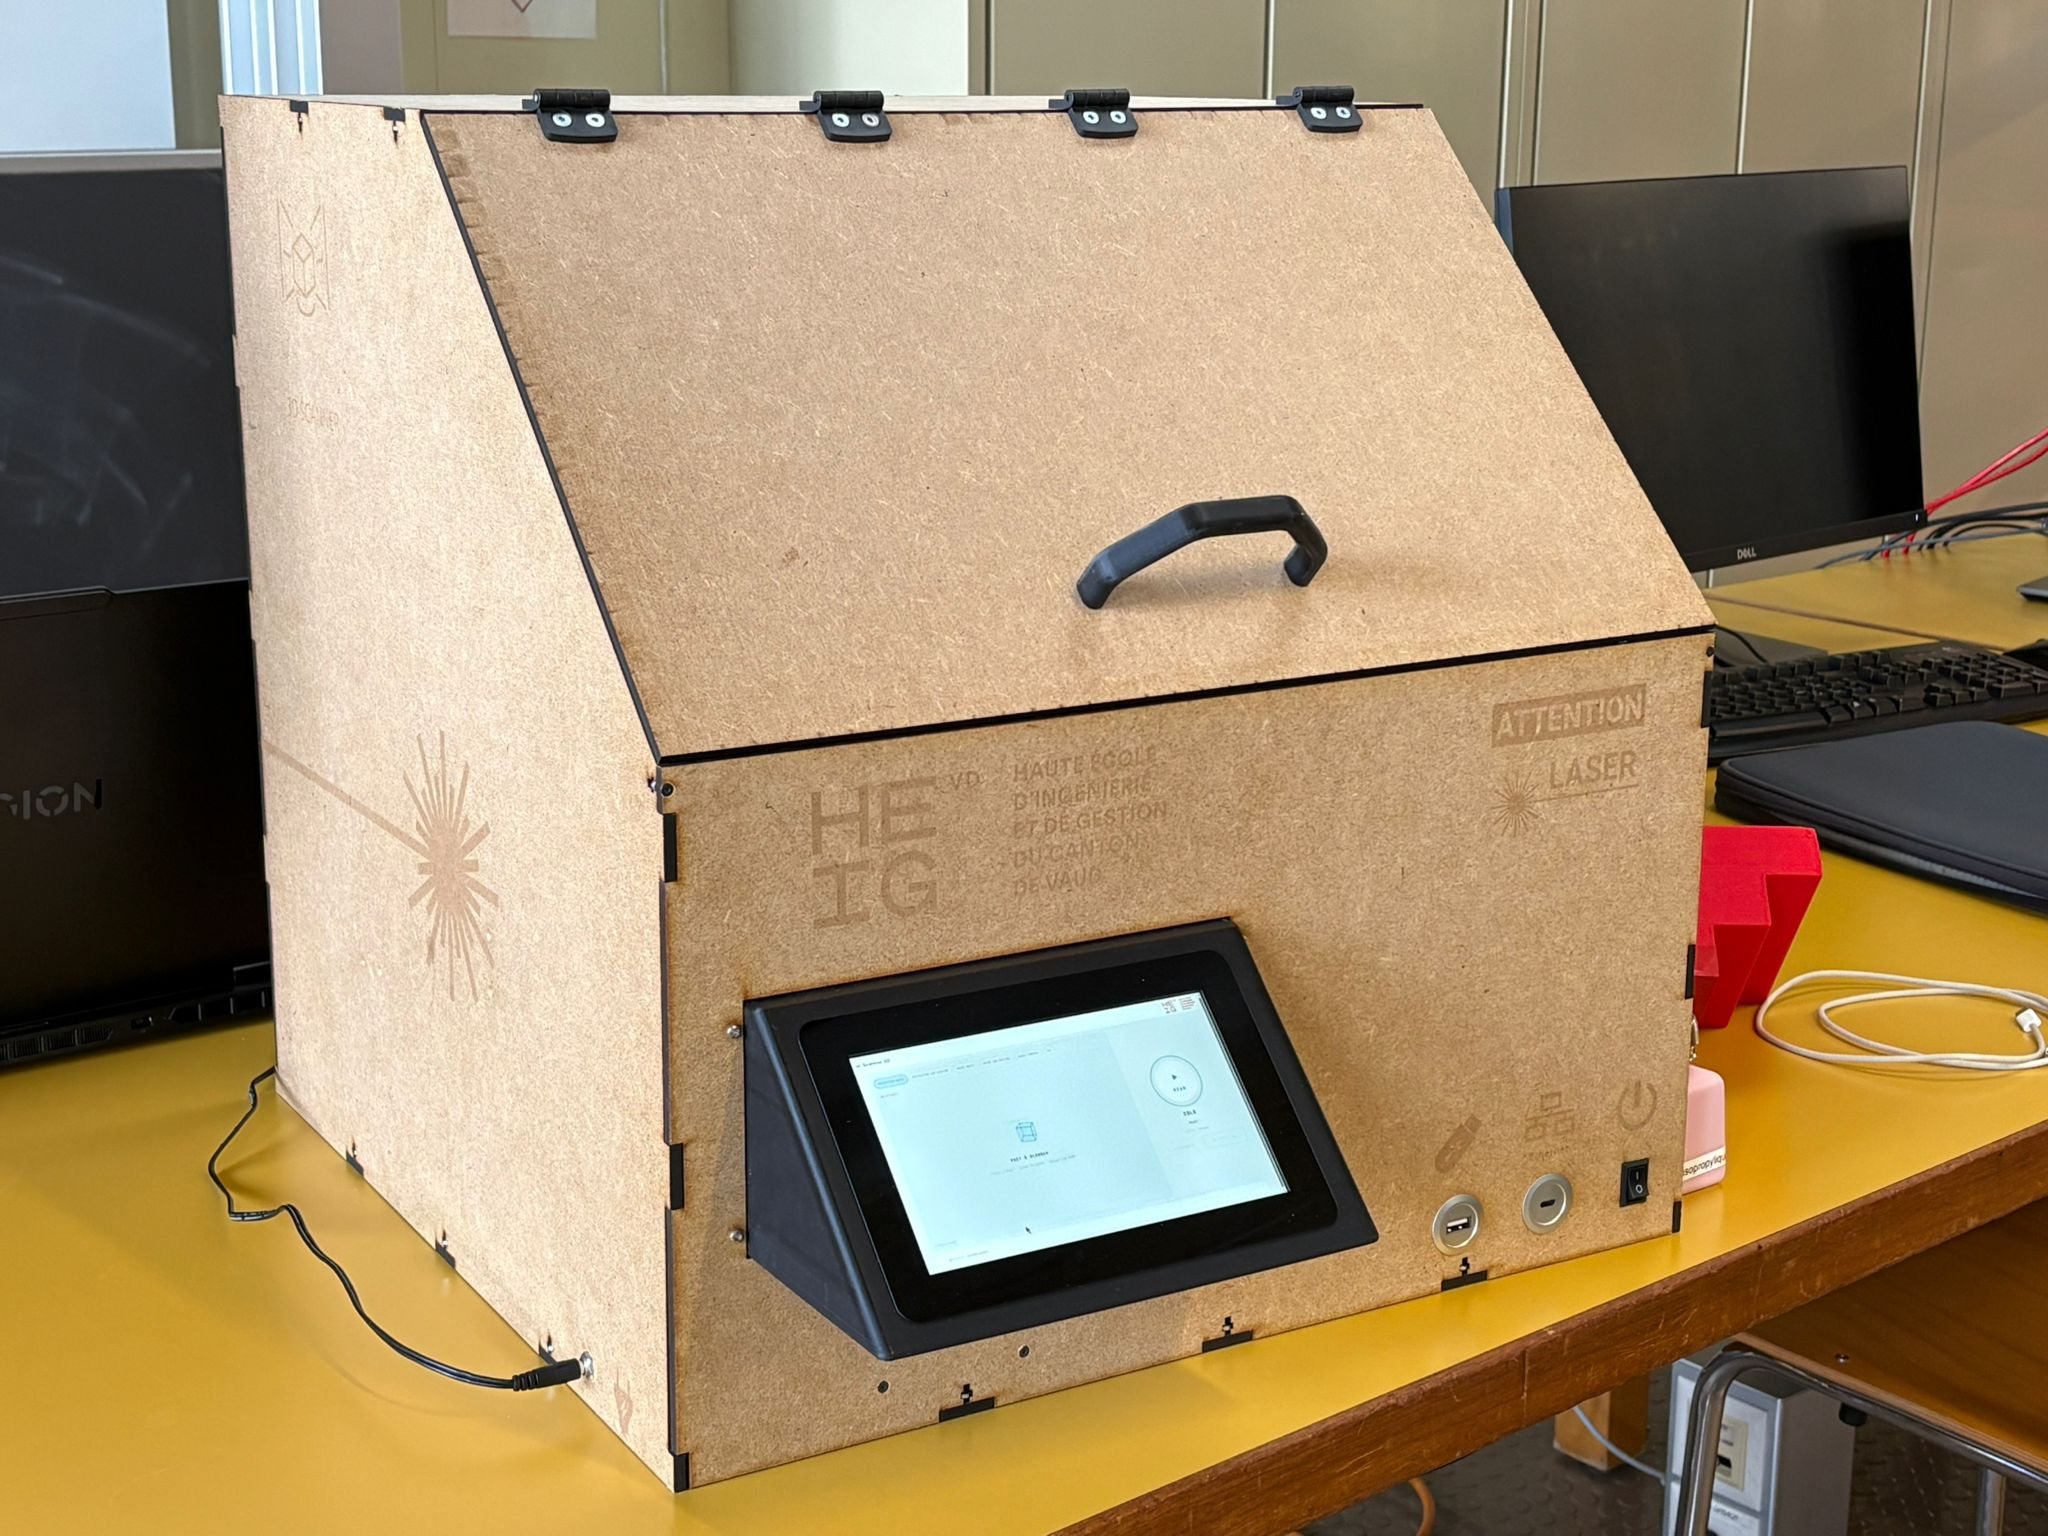
\includegraphics[width=7.3cm,height=4.75cm,keepaspectratio]{boitefinal.jpeg}};
    \node[anchor=south east,inner sep=0pt] at ([xshift=-0.62cm,yshift=0.84cm]current page.south east)
      {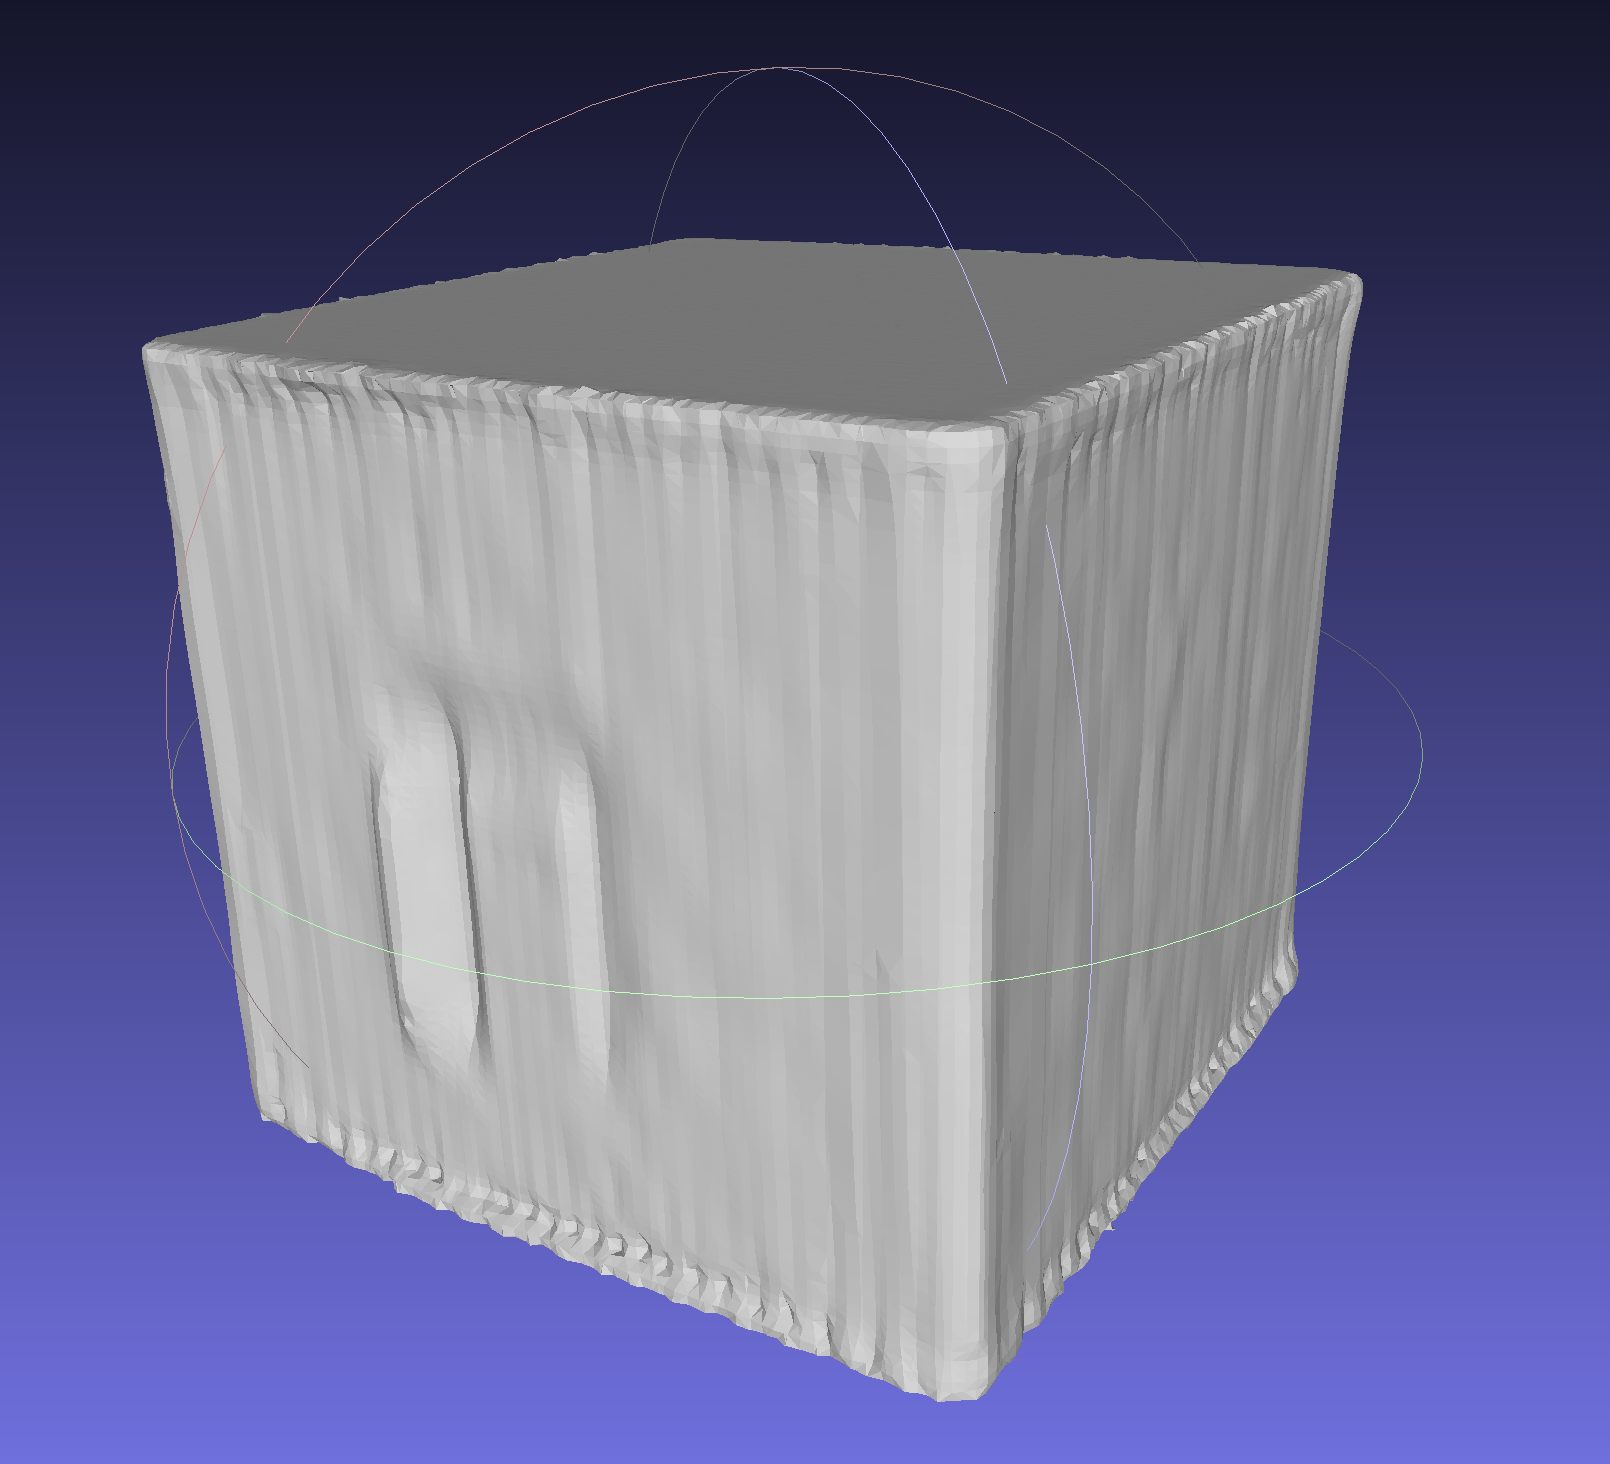
\includegraphics[width=5.40cm,height=2.45cm,keepaspectratio]{cube.png}};
  \end{tikzpicture}
\end{frame}

% 2
\begin{frame}[plain]
  \slidetitle{Objectif}
  \begin{columns}[T,totalwidth=14.5cm]
    \begin{column}{0.48\linewidth}
      \vspace{0.18cm}
      \begin{itemize}
        \item Numériser un objet réel dans une boîte fermée et sécurisée.
        \item Acquérir un profil laser à chaque angle du plateau.
        \item Transformer les pixels laser en points 3D calibrés.
        \item Exporter un nuage de points et un modèle STL imprimable.
      \end{itemize}
      \vspace{0.42cm}
      \redtag{CIBLE} \quad 100 vues sur 360° avec double caméra
    \end{column}
    \begin{column}{0.49\linewidth}
      \begin{tikzpicture}[node distance=0.42cm]
        \tikzstyle{processbox}=[draw=ink,line width=0.75pt,minimum width=5.9cm,minimum height=0.64cm,align=left,inner xsep=7pt,font=\small]
        \node[processbox] (laser) {\textbf{Laser} : ligne verte sur l'objet};
        \node[processbox,below=of laser] (cams) {\textbf{Caméras} : image droite + image gauche};
        \node[processbox,below=of cams] (pix) {\textbf{Extraction} : 1 point laser par ligne image};
        \node[processbox,below=of pix] (tri) {\textbf{Triangulation} : pixels $\rightarrow$ profil 3D};
        \node[processbox,below=of tri] (mesh) {\textbf{Export} : PLY + STL / OBJ};
        \draw[-{Latex[length=2.2mm]},heigred,line width=0.9pt] (laser) -- (cams);
        \draw[-{Latex[length=2.2mm]},heigred,line width=0.9pt] (cams) -- (pix);
        \draw[-{Latex[length=2.2mm]},heigred,line width=0.9pt] (pix) -- (tri);
        \draw[-{Latex[length=2.2mm]},heigred,line width=0.9pt] (tri) -- (mesh);
      \end{tikzpicture}
    \end{column}
  \end{columns}
\end{frame}

% 3
\begin{frame}[plain]
  \slidetitle{Architecture}
  \begin{columns}[T,totalwidth=14.5cm]
    \begin{column}{0.49\linewidth}
      \imagebox{width=6.65cm,height=4.45cm,keepaspectratio}{montage2camera.jpeg}
      \vspace{0.18cm}
      {\small\color{muted}Deux points de vue réduisent les occultations et permettent de fusionner les profils.}
    \end{column}
    \begin{column}{0.48\linewidth}
      \vspace{0.08cm}
      \metric{2}{caméras calibrées}
      \metric{100}{positions par tour}
      \metric{16}{micro-pas moteur}
      \vspace{0.62cm}
      \begin{itemize}
        \item Plateau NEMA 17 piloté par STEP/DIR.
        \item Laser coupé après chaque capture.
        \item Interlock porte : arrêt immédiat si la boîte s'ouvre.
        \item Interface web pour lancer, suivre et récupérer les fichiers.
      \end{itemize}
      \vspace{0.15cm}
      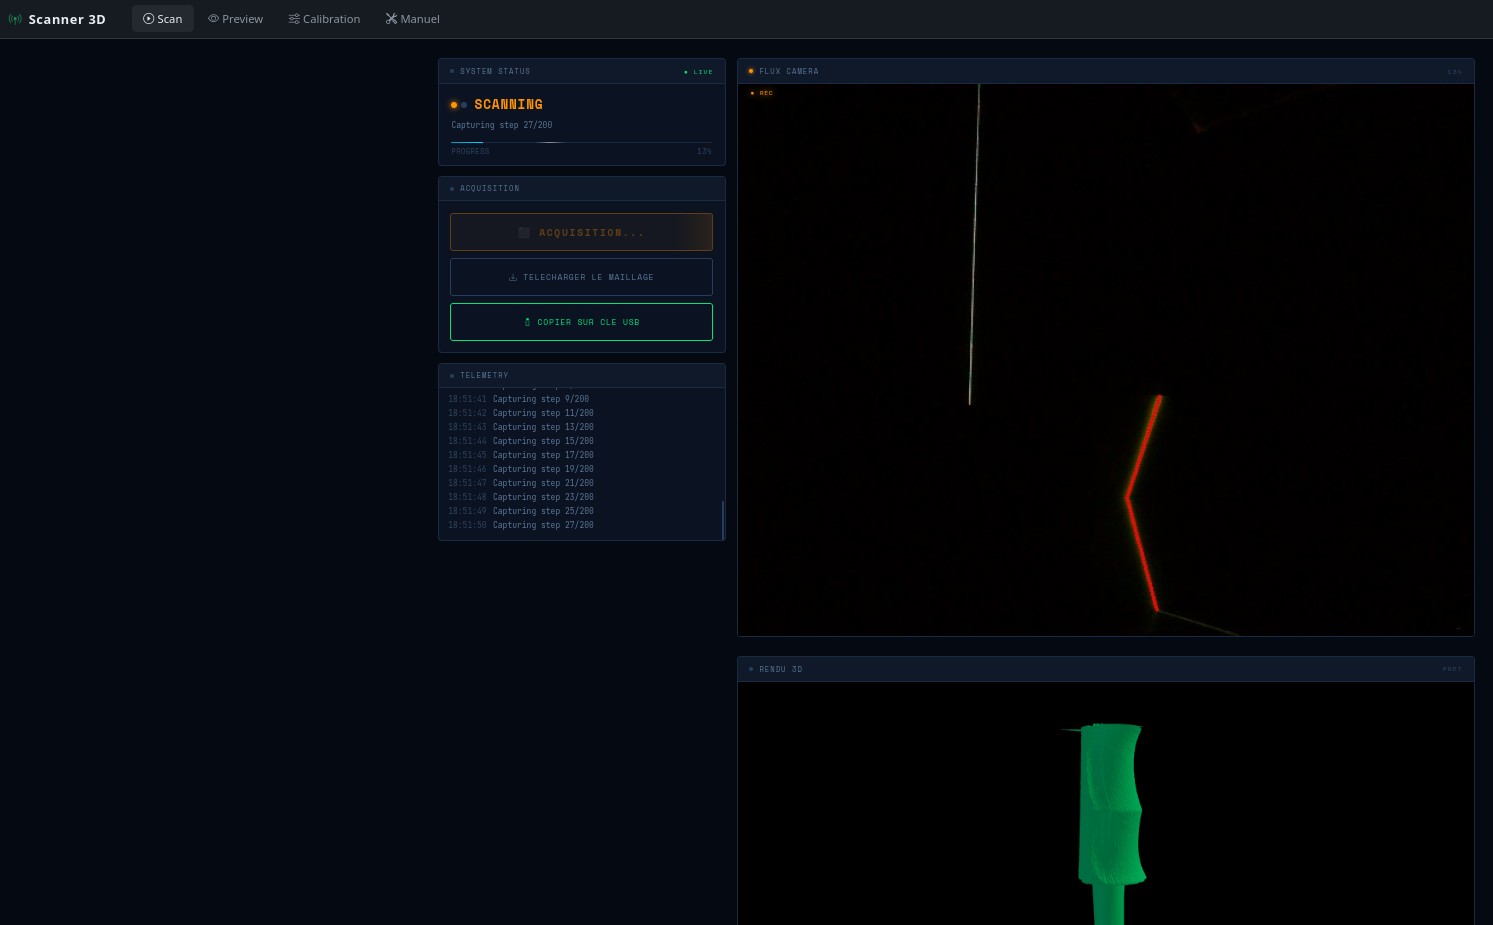
\includegraphics[width=5.7cm,height=1.55cm,keepaspectratio]{screen_interface.png}
    \end{column}
  \end{columns}
\end{frame}

% 4
\begin{frame}[plain]
  \slidetitle{Méthode logicielle}
  \begin{columns}[T,totalwidth=14.5cm]
    \begin{column}{0.47\linewidth}
      \begin{tikzpicture}[x=1cm,y=1cm]
        \draw[->,linegray] (0,0) -- (6.1,0) node[right,font=\scriptsize] {angle};
        \draw[->,linegray] (0,0) -- (0,3.35) node[above,font=\scriptsize] {profil};
        \foreach \x/\h in {0.35/1.0,1.1/2.2,1.85/2.65,2.6/1.9,3.35/2.45,4.1/1.55,4.85/2.0,5.6/0.9}{
          \draw[heigred,line width=1.25pt] (\x,0.18) -- (\x,\h);
          \fill[heigred] (\x,\h) circle (1.2pt);
        }
        \node[anchor=west,font=\bfseries] at (0.25,3.12) {Profils laser successifs};
        \node[font=\small] at (1.2,-0.34) {capture};
        \node[font=\small] at (3.1,-0.34) {triangulation};
        \node[font=\small] at (5.0,-0.34) {fusion};
      \end{tikzpicture}
      \vspace{0.35cm}
      \begin{itemize}
        \item Seuil sur le canal vert, puis centroïde par ligne image.
        \item Rayon caméra + plan laser = point 3D du profil.
        \item Dérotation par l'angle du plateau dans le repère objet.
      \end{itemize}
    \end{column}
    \begin{column}{0.49\linewidth}
      \begin{beamercolorbox}[wd=\linewidth,sep=0.16cm]{normal text}
      {\small\ttfamily
      frames = run\_capture\_sequence\_multi()\\
      line = extract\_laser\_line(frame)\\
      pts = triangulate(line, camera, plane, angle)\\
      profile = fuse\_step\_profiles(pts\_by\_camera)\\
      cloud = merge\_profiles(profiles)\\
      export\_stl(cloud, output)}
      \end{beamercolorbox}
      \vspace{0.34cm}
      \redtag{POINT CLÉ} \quad géométrie reconstruite depuis la calibration
      \vspace{0.32cm}

      {\small
      \textbf{100 vues} \quad \textbf{4 px min.} \quad \textbf{20 voisins} \quad \textbf{STL}}
      \vspace{0.08cm}

      {\scriptsize\color{muted}Paramètres lus dans le code et la configuration courante.}
    \end{column}
  \end{columns}
\end{frame}

% 5
\begin{frame}[plain]
  \slidetitle{Résultats + vidéo}
  \begin{columns}[T,totalwidth=14.5cm]
    \begin{column}{0.51\linewidth}
      \begin{tikzpicture}
        \node[inner sep=0pt] at (0,0) {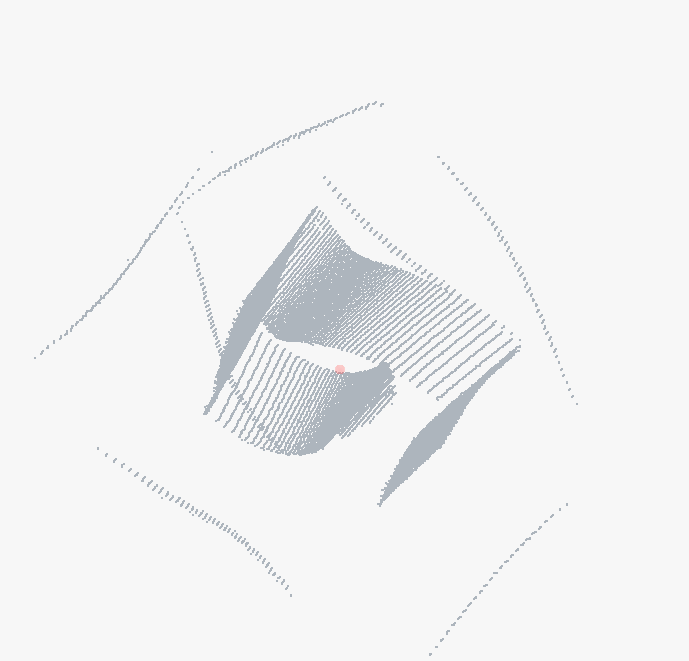
\includegraphics[width=3.15cm,height=3.15cm,keepaspectratio]{carre_nuage.png}};
        \node[inner sep=0pt] at (3.25,0) {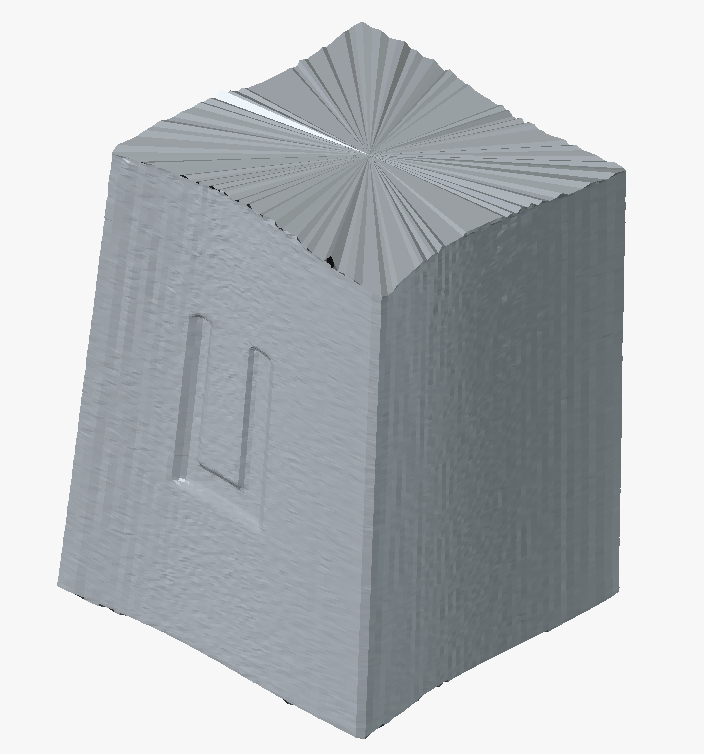
\includegraphics[width=3.15cm,height=3.15cm,keepaspectratio]{carre_gris_stl.png}};
        \node[inner sep=0pt] at (0,-3.25) {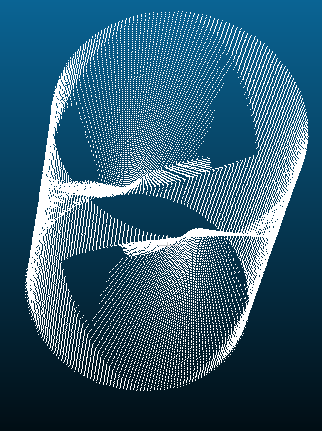
\includegraphics[width=3.15cm,height=3.15cm,keepaspectratio]{screen_cylindre_nuage.png}};
        \node[inner sep=0pt] at (3.25,-3.25) {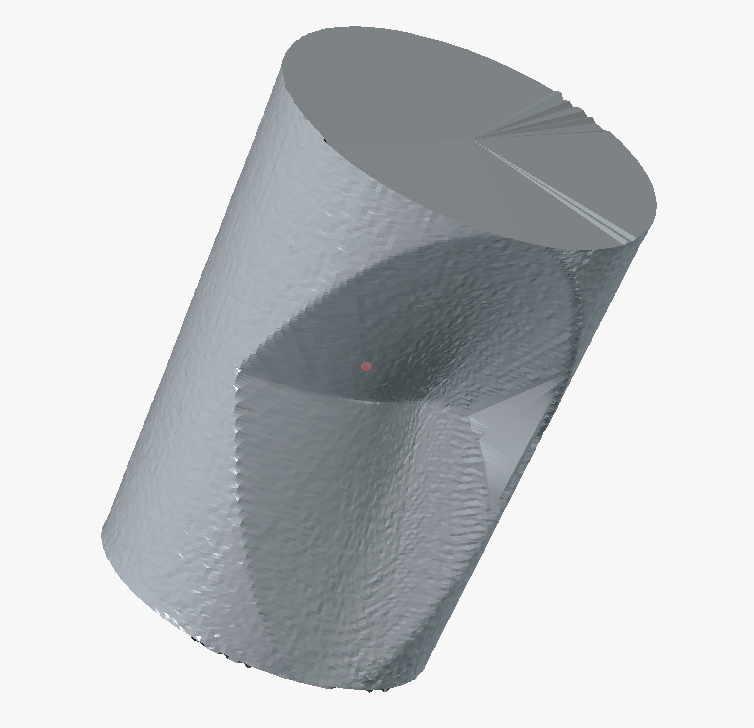
\includegraphics[width=3.15cm,height=3.15cm,keepaspectratio]{screen_cylindre_stl.png}};
        \draw[heigred,line width=1.2pt] (-1.58,-1.68) -- (1.0,-1.68);
      \end{tikzpicture}
    \end{column}
    \begin{column}{0.46\linewidth}
      \begin{tabular}{@{}ccc@{}}
        \makebox[1.8cm][c]{{\fontsize{19}{21}\selectfont\bfseries PLY}} &
        \makebox[1.8cm][c]{{\fontsize{19}{21}\selectfont\bfseries STL}} &
        \makebox[1.8cm][c]{{\fontsize{19}{21}\selectfont\bfseries OBJ}} \\
        \parbox[t]{1.8cm}{\centering\scriptsize\color{muted}nuage brut} &
        \parbox[t]{1.8cm}{\centering\scriptsize\color{muted}maillage} &
        \parbox[t]{1.8cm}{\centering\scriptsize\color{muted}export web}
      \end{tabular}
      \vspace{0.48cm}
      \begin{tikzpicture}
        \draw[fill=soft,draw=linegray,line width=0.8pt] (0,0) rectangle (6.1,2.35);
        \node[align=center,font=\bfseries\large] at (3.05,1.45) {Vidéo démo};
        \node[align=center,font=\small,color=muted] at (3.05,0.86) {35 s intégrées au timing};
        \node[align=center,font=\scriptsize,color=muted] at (3.05,0.34) {Ajouter \texttt{assets/video\_35s.mp4} si disponible};
      \end{tikzpicture}
      \IfFileExists{assets/video_35s.mp4}{%
        \vspace{-2.45cm}
        \movie[width=6.1cm,height=2.35cm,poster,showcontrols]{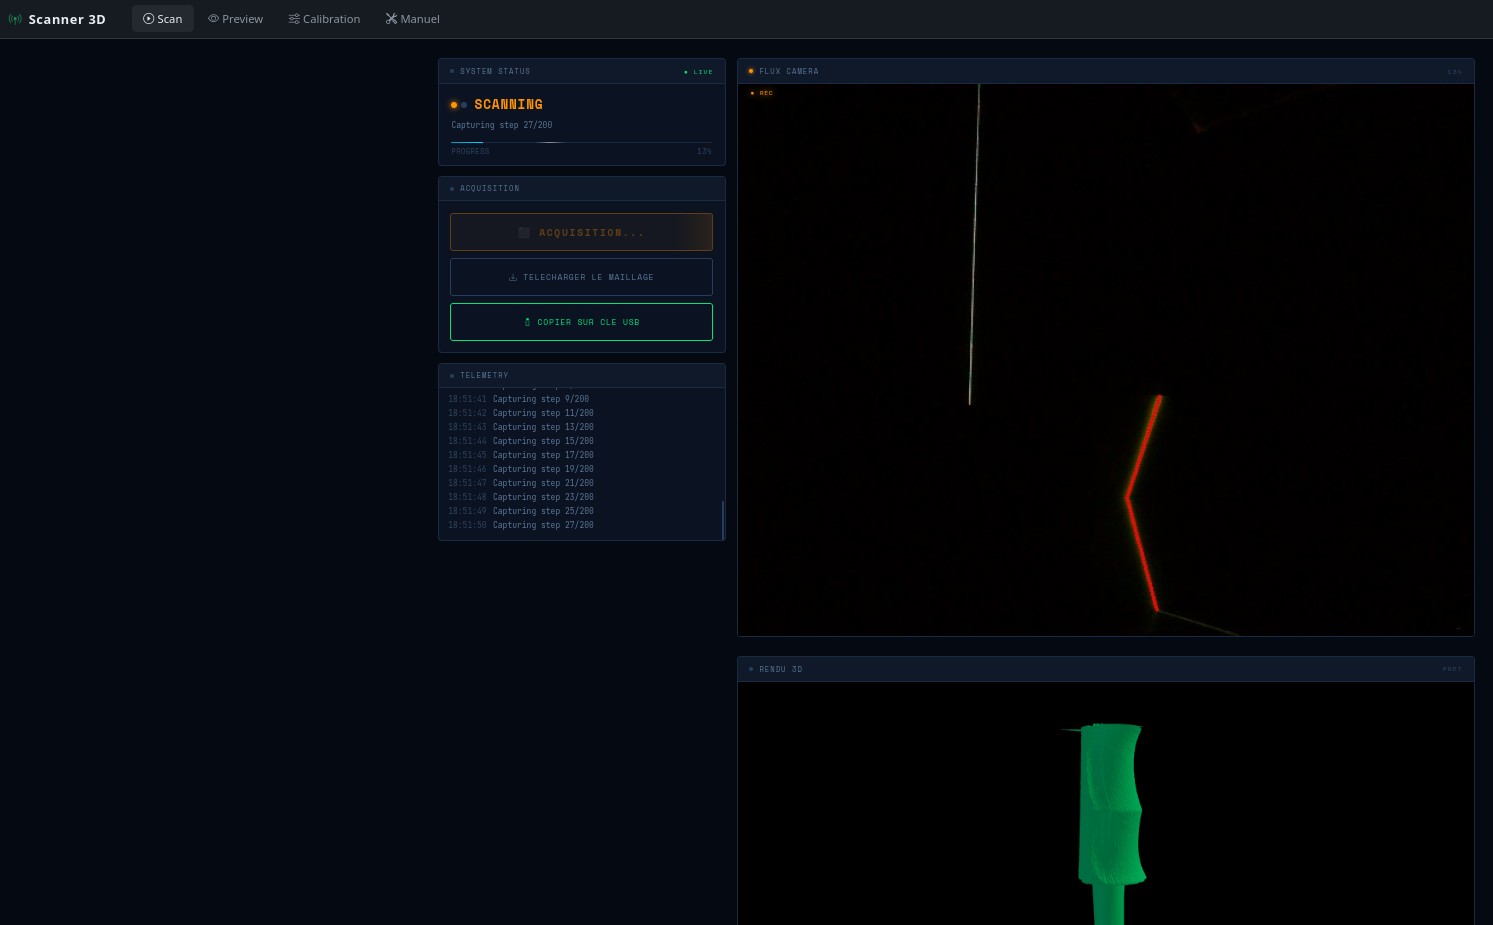
\includegraphics[width=6.1cm,height=2.35cm]{screen_interface.png}}{assets/video_35s.mp4}
      }{}
      \vspace{0.25cm}
      {\small\color{muted}Le résultat important : la chaîne ne s'arrête pas au nuage, elle produit un fichier exploitable.}
    \end{column}
  \end{columns}
\end{frame}

% 6
\begin{frame}[plain]
  \slidetitle{Résumé final}
  \begin{columns}[T,totalwidth=14.5cm]
    \begin{column}{0.45\linewidth}
      \imagebox{width=6.2cm,height=4.35cm,keepaspectratio}{vue_interieur_laser_piece.jpeg}
      \vspace{0.16cm}
      {\small\color{muted}La partie critique est la cohérence entre mécanique, calibration et traitement.}
    \end{column}
    \begin{column}{0.51\linewidth}
      \vspace{0.12cm}
      \begin{itemize}
        \item Acquisition automatisée : moteur, laser, deux caméras, sécurité porte.
        \item Traitement reproductible : extraction laser, triangulation, fusion des profils.
        \item Résultat exporté : nuage PLY et maillage STL / OBJ.
        \item Limite actuelle : qualité dépendante de la calibration et des occultations.
      \end{itemize}
      \vspace{0.45cm}
      {\fontsize{22}{25}\selectfont\bfseries D'une ligne laser à un objet imprimable.}
      \vspace{0.28cm}

      
\includegraphics[height=0.55cm]{logo_hesso.pdf}
    \end{column}
  \end{columns}
\end{frame}

\end{document}
